\begin{refsection}
\chapter{Введення в лапароскопічну хірургію печінки}
\section{Історія розвитку методики}
\subsection{Перший досвід}
Мініінвазивні втручання радикально змінили хірургічну практику за останні три десятиріччя та призвели до суттєвого покращення результатів за рахунок зменшення частоти післяопераційних ускладненнь, тривалості госпіталізації та співвідношення вартості до еффективності лікування в різних хірургічних спеціальностях, включаючи колоректальну хірургію, урологію, гінекологію та торокальну хірургію. Природньо, що зацікавленість хірургів в лапароскопічному доступі швидко розповсюдилась на гепатобіліарні втручання, спроби виконання яких в лапароскопічному варіанті було розпочато в 1987 році із першої лапароскопічної холецистектомії \cite{Litynski}. 

Для лікування уражень печінки лапароскопія була вперше впроваджена на початку 90х. Будучи широковживаною в загальній хірургії, в печінковій хірургії лапароскопія зіткнулась із багатьма перешкодами, проте переваги лапароскопічного доступу, такі як покращена візуалізація, та зменшення післяопераційних ускладненнь  надали стимул для розвитку лапароскопічних резекцій печінки (\acrshort{llr}). Перші резекції печінки в лапароскопічному варіанті були виконані в 1991 році Reich H. \cite{Reich1991a} та  в 1992 Katkhouda N. \cite{Katkhouda1992} та Gagner M. \cite{GAGNER1992}. Ці операції були крайовими резекціями невеликих, переважно доброякісних новоутворень, проте невдовзі стало зрозуміло, що результати лапароскопічних операцій порівняні із традиційними відкритими втручаннями а \acrshort{llr} є безпечним та ефективним методом лікування. Відтоді \acrshort{llr} стала потенційною альтернативою відкритій резекції печінки (\acrshort{olr}). 
На початку розвиток методики був повільним, і наступні декілька років публікації містили лише опис поодиноких випадків атипових резекцій \cite{Klotz1993, Cunningham1995}. Перша анатомічна лапароскопічна лівобічна латеральна секцієектомія(\acrshort{llls}) виконана в 1996 році \cite{Azagra1996}  відновила інтерес до \acrshort{llr} не дивлячись на те, що перші випадки анатомічних резекцій були конвертовані у відкриті втручання через масивну інтраопераційну кровотечу \cite{Hashizume1995}.  Із накопиченням досвіду покази до \acrshort{llr} були розширені до гемігепатектомій, складних сегментектомій, трисекцієектомій та навіть донорських резекцій при трансплантації печінки від живого донора \cite{Dagher2009, Cherqui2002, Jia2018}. 

\subsection{Погоджувальні конференції}

Від моменту виконання першої \acrshort{llr} кількість публікацій присвячених темі щорічно прогресивно збільшується (Рис. \ref{fig:plot1}). Стимулом до цього є посітйне вдосконалення ендохірургічного обладнання та хірургічної техніки.
Аккумуляція досвіду поставила перед хірургічною спільнотою завдання відповіді на ключові питання пов'язані з \acrshort{llr}: по-перше це безпека та відтворюваність методики а по-друге її онкологічна ефективність. Для відповіді на них та створення клінічних рекомендацій стосовно застосування \acrshort{llr} було послідовно проведено декілька погоджувальних конференцій, висновки яких відображують процес становлення лапароскопічного методу та зміну відношення до нього хірургічного загалу. 

\begin{figure}[h]
\caption{Динаміка кількості публікацій в PubMed по запиту "laparosopic liver resection" по роках}
\centering
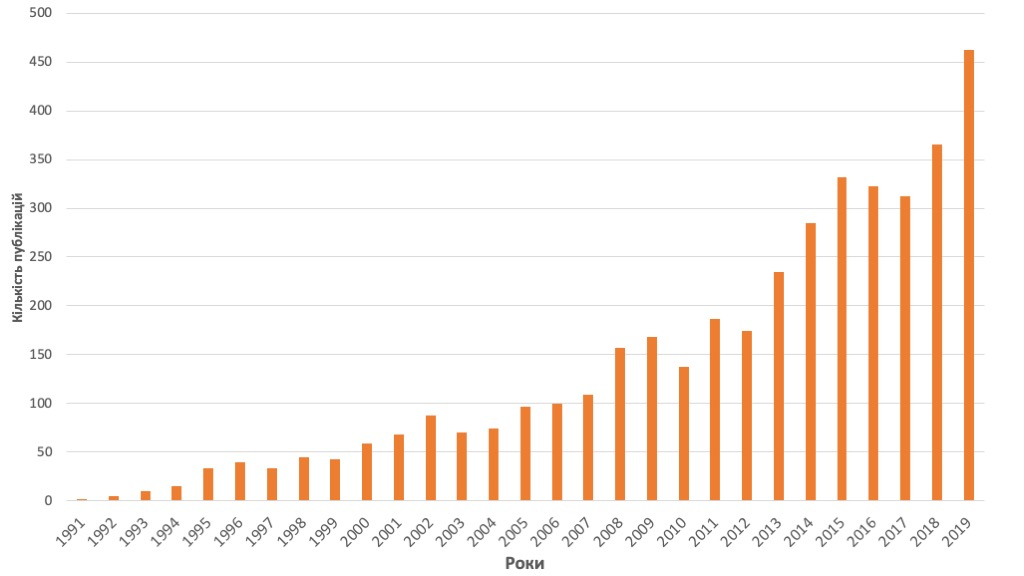
\includegraphics[width=0.9\textwidth]{Illustrations/Pic_01.jpg}
\label{fig:plot1}
\end{figure}

\subsubsection{Перша погоджувальна конференція} 

Перша погоджувальна конференція відбулась в Луізвілі в листопаді 2008 року за участі 45 міжнародних експертів з гепатобіліарної хірургії. \cite{Buell2009}. За результатами обговорення до  \acrshort{llr} були віднесені чисто лапароскопічні, хенд-асистовані резекції печінки (\acrshort{hals}) та гибридні резекції печінки (\acrshort{hlr}) при яких початкова диссекція проводиться в лапароскопічному варіанті а розсічення паренхіми через мінілапаротомію. 

Прийнятними для видалення за допомогою  \acrshort{llr} були визначені утворення, розміром менше 5 см, що розташовані в 2 - 6 сегментах печінки, а \acrshort{llls} було рекомендовано розглядати в якості стандартної практики. Також була показана принципова технічна можливість видалення новоутворень, локалізованих в будь яких сегментах печінки в лапароскопічному варіанті, проте обширні резекції печінки було рекомендовано зарезервувати за спеціалізованими гепатобіліарними центрами з великим досвідом як лапароскопічних втручаннь, так і резекційної хірургії печінки. 

Конверсію рекомендовано розглядати скоріше як необхідний крок для безпечного завершення складного втручання, ніж як ускладнення. Перед ургентною конверсією з приводу кровотечі хірург повинен докласти максимальних зусиль до зупинки кровотечі лапароскопічними методами. 

Вперше була показана можливість виконання донорського забору печінки при трансплантації від живого донора у дітей в лапароскопічному варіанті. Донорську \acrshort{llls} було оцінено, як експериментальну методику, що має великий потенціал але потребує детального вивчення. 

Вцілому консенсус визначив \acrshort{llr} як безпечну альтернативу традиційним резекціям та рекомендував методику до подальшого вивчення та більш широкого впровадження досвідченими гепатобіліарними хірургами.

\subsubsection{Друга погоджувальна конференція} 

На відміну від першої, друга погоджувальна конференція, яка відбулась в японському місті Моріока в жовтні 2014 році \cite{Kaneko2015}, була побудована за Цюріхсько-Датською моделлю, та включала в себе експертну панель з 43 досвідчених хірургів та 9 членів жюрі з 18 країн які оцінювали результати \acrshort{llr}. Для оцінки були запропоновані 17 запитаннь в категоріях переваги, ризики та технічні аспекти \acrshort{llr}, відповідаючи на які жюрі сформувало рекомендації. Доказова якість рекомендацій була оцінена за шкалою GRADE а ступінь розробки втручаннь за системою IDEAL \cite{Guyatt2008, McCulloch2009}. Для об'єму резекції було запропоноване класичне визначення: до малих резекцій (Minor resection) було віднести резекції 2 та меньше сегментів а до великих або обширних (Major resection) 3 та більше сегментів. Але зважаючи на те, що технічна складність \acrshort{llls} та правобічної задньої або передньої секцієектомії в лапароскопічному варіанті значно відрізняються, резекції, до складу яких входять сегменти 7 або 8 було віднесено до великих. 

За висновками експертного жюрі як малі так і великі \acrshort{llr} не гірші за відкриті в показниках операційної летальності, післяопераційних ускладненнь, чистоті резекційного краю, загальної виживаності та вартості операції та мають перевагу в більш короткому терміні перебування в стаціонарі, меншій крововтраті. Експерти погодились з тим, що результати лапароскопічних донорських заборів не відрізнялись від відкритих у високоспеціалізованих центрах. У якості додаткового висновку жюрі заключило, що великі \acrshort{llr} вимагають високого рівню хірургічних навичок та тривалої кривої навчання.

Основними досягненнями конференції було по-перше визнання того, що  \acrshort{llr} за більшістю показників не поступаються, а за окремими показниками перевершують відкриті втручання, а по-друге рекомендація використовувати малі \acrshort{llr} в якості стандарту надання допомоги.

\subsubsection{Створення клінічних рекомендацій} 
Подальший еспотенціальний ріст кількості \acrshort{llr} призвів до того, що в лютому 2017 року в Саузхемптоні була проведена третя погоджувальна конференція \cite{AbuHilal2017a} яка мала на меті створення загальноєвропейських клінічних рекомендацій. В процесі підготовки було залучено експертну панель з 11 досвідчених гепатобіліарних хірургів, частина з яких мала досвід лише відкритих резекцій печінки а частина як відкритих так і \acrshort{llr}. Після аналітичного обзору 647 джерел, відібраних за допомогою критеріїв включення експертами були сформовані рекомендації в п'яти ключових напрямках: покази, відбір пацієнтів, види втручаннь, технічні особливості та імплементація.

Згідно з цими рекомендаціями \acrshort{llr} показані для лікування метахронних колоректальних метастазів та гепатоцеллюлярної карциноми так як ассоційовані зі зниженням крововтрати, післяопераційного асциту, печінкової недостатності та терміну перебування в стаціонарі порівняно із відкритими втручаннями при порівняній тривалості операції, частоті R0 краю резекції та рівні рецидивів. Також \acrshort{llr} показані для лікування доброякісної вогнищевої патології завдяки суттєвому зниженню післяопераційних ускладненнь, больового синдрому та терміну перебування в стаціонарі, що підтверджено на великих серіях пацієнтів, у тому числі із великими резекціями. Донорські гепатектомії наразі не є добре стандартизованими процедурами та зарезервовані за високоспеціалізованими центрами.

Що до відбору пацієнтів, то \acrshort{llr} добре показали себе у хворих з вираженою коморбідністю та можуть бути рекомендовані для пацієнтів з ожирінням та пацієнтів старшого віку. Є данні, що свідчать про полегшення перебігу повторних (відкритих або лапароскопічних) резекцій печінки у пацієнтів, що перенесли \acrshort{llr} в якості первинної операції. Складні випадки з великими новоутвореннями (> 10 см) та близкістю до магістральних судин не є протипоказами до \acrshort{llr}, так як можуть бути виконані з аналогічною відкритим операціям  морбідністю.

Усі види \acrshort{llr}, як великі так і малі, асоційовані зі зменшенням інтраопераційної крововтрати, післяопераційних ускладненнь та терміну перебування в стаціонарі та аналогічними показниками онкологічної результативності порівняно з віткритими втручаннями. Великі втручання та втручання на задніх сегментах пов'язані із більшою складністю та тривалістю операції, проте в експертних центрах можуть бути досягнуті периопераційні результати аналогічні малим \acrshort{llr}.

Також в рекомнедаціях зазначено, що жодна з існуючих технік виконання \acrshort{llr} (\acrshort{hals}, \acrshort{hlr} або чисто лапароскопічна) не показала абсолютної переваги над іншими, проте вважається, що \acrshort{hals} та \acrshort{hlr} є перехідними до чисто лапароскопічної техніки. Те ж саме стосується й техніки транссекції паренхіми: краш-кламп, використання CUSA або інших хірургічних енергій визнано рівноцінними методами. Для диссекції портальних структур більшисть хірургів використовують ізольоване лігування, проте глісоновий підхід показав аналогічні результати. Для контролю кровотечі під час \acrshort{llr} рекомендовано використовувати лапароскопічний прийом Прінгла та анастезію з низьким центральним венозним тиском (\acrshort{cvp}). Факторами ризику конверсії на відкрите втручання є високий індекс маси тіла, розмір пухлини, локалізація ураження в постеролатеральних сегментах та цирроз. Перед виконанням ургентної конверсії рекомендовано досягти тимчасового гемостаза лапароскопічними методами.

Крива навчання малих \acrshort{llr} складає 60 випадків для хірурга, що має досвід відкритих резекцій печінки. Для великих \acrshort{llr} цей показник становить 55 операцій, при умові успішного проходження кривої для малих \acrshort{llr}. Впровадження \acrshort{llr} не повинно відбуватись в ізоляції від відкритої хірургії печінки. Для кожного спелізованого гепатобіліарного центру рекомендована наявність не менше двох хірургів, спеціалізованих на \acrshort{llr}.

Якщо послідовно проаналізувати висновки всіх погоджувальних конференцій стає зрозумілим, що методика \acrshort{llr} успішно пройшла крізь етапи розробки, первинної оцінки результатів та широкого впровадження базуючись на принципах доказової медицини. Чисельна кількість дослідженнь на великих групах пацієнтів \cite{Ciria2016b, Takahara2016, Berardi2017}, в тому числі два рандомізоаних клінічних дослідження \cite{Fretland2018b, Robles-Campos2019} свідчать про перевагу \acrshort{llr} над традиційними відкритими втручаннями в періопераційних показниках зі збереженням онкологічної ефективності. 

\section[Сучасні можливості]{Сучасні можливості лапароскопічної резекційної хірургії печінки}

\subsection{Анатомічні резекції печінки}
З моменту першої \acrshort{llr} можливості методу значно поширились за межі крайових резекцій новоутворень невеликого розміру. На данний момент показана доступність виконання в лапароскопічному варіанті абсолютно всіх видів анатомічних резекцій печінки при доброякісних та онкологічних пухлинах, включно навіть з операціями при хіларній холангіокарциномі. Найбільш часто вживані резекції, такі як \acrshort{llls}, лівобічна та правобічна гемігепатектомія та моносегментектомії є добре вивченими та стандартизованими процедурами, що дозволяє деяким спеціалізованим центрам \cite{Garbarino2019} виконувати до 80-90\% всіх резекцій печінки в лапароскопічному варіанті. Тож, в більшості випадків, вибір доступу визначається скоріше можливостями клініки ніж можливостями методики. 

За об'ємом розрізняють малі (Minor) та великі або обширні (Major) резекції. До малих резекцій відносять моно- та бісегментектомії антеролатеральних сегменітв та ліву латеральну секцієектомію. До великих або обширних анатомічних \acrshort{llr} відностяь резекції при яких виляляють три або більше розташованих поруч сегмента. Класичними представниками великих резекцій є лівобічна та правобічна гемігепатектомії.

\subsubsection{Лівобічна гемігепатектомія}

Лапароскопічна лівобічна гемігепатектомія (\acrshort{llhe}) показала себе як доступна, безпечна та ефективна процедура для пацієнтів, що мають новоутворення лівої долі печінки. В ретроспективному порівняльному аналізі 62 \acrshort{llhe} та 118 відкритих лівобічних гемігепатектомій у пацієнтів з гепатоцеллюлярною карциномою (\acrshort{hcc}), внутрішньопечінковою холангіокарциномою (\acrshort{ihcc}) та деякими доброякісними новоутвореннями показано перевагу лапароскопічних втручаннь за рахунок зменшення крововтрати, часу до відновлення харчування та частоти важких ускладненнь з порівняними показниками виживаності у онкологічних хворих \cite{Cho2018b}.   Міжнародне мультицентрове ретроспективне дослідження реузльтатів 82 \acrshort{llhe} \cite{Belli2013a} не виявило достовірної різниці кількості ускладненнь та періопераційних показників у порівнянні з 222 \acrshort{llls}, - процедурою, яка є визнаним "золотим стандартом". Не дивлячись на те, що \acrshort{llhe} є технічно складнішою за \acrshort{llls}, автори рекомендують її в якості стандартного методу лікування.

\subsubsection{Правобічна гемігепатектомія}

Лапароскопічна правобічна гемігепатектомія (\acrshort{lrhe}) є непростим втручанням, так як потребує повної мобілізації та маніпуляцій з об'ємною правою долею печінки, що потребує технічної майстерності від оперуючого хірурга. З моменту першого виконання Hüscher C. в 1995 році \cite{Huscher1997} техніка \acrshort{lrhe} вдосконалювалась та зазнавала постійних модифікацій \cite{Gayet2007, Dagher2008, Homma2019, Kim2017a}. В сучасному варіанті \acrshort{lrhe} є добре вивченою процедурою. Її онкологічна еффективність та рівень ускладнень у пацієнтів з ГЦК на фоні цирозу не відрізняється від традиційної відкритої правобічної гемігепатектомії за результатами корейського моноцентрового ретроспективного псевдорандомізованого дослідження \cite{Yoon2017b}. 

\subsubsection{Секцієектомії та центральні резекції}

Окрім \acrshort{llhe} та \acrshort{lrhe} обширні резекції включають в себе праву передню, праву задню та ліву медіальну секцієектомії, мезогепатектомію. Технічно такі операції вважаються складнішими за класичні гемігепатектомії, так як включають дві площини резекції, що знаходяться під кутом одна до одної. Не дивлячись на це, в серії дослідженнь показано, що такі втручання є безпечними та відтворюваними в експертних центрах \cite{Honda2014, Cheng2015, Kim2017, Siddiqi2018}. 

\subsubsection{Складні локалізації}

Постерокраніальні сегменти (Sg 7,8) та каудальна лобектомія певний час вважались недоступними для лапароскопічного доступу через високе незручне розтажування обмежене ребрами та куполом діафрагми, та анатомічну близкість до печінкових вен та нижньої порожнистої вени (\acrshort{ivc}). В 2014 роци Ban D. та співавтори розробили шкалу складності для \acrshort{llr}, де віднесли ізольовані лапароскопічні резекції Sg 7 та 8 до резекцій вищого ступеню складності, порівняно з резекціями інших анатомічних ділянок. Для полегшення доступу до постерокраніальних сегментів Ikeda T. була запропонована напівпронована позиція пацієнта та латеральний доступ до Sg 7-8 \cite{Ikeda2014}. Пізніше Honda G. та співавторами була опублікована методика анатомичної резекції Sg 7 з внутрішньопечінковим доступом до сегментарного  гліссону \cite{Okuda2017}, а Inoue Y. показано спосіб резекції Sg 6, 7 та 8 з латерального доступу з використанням трансторакальних троакарів \cite{Inoue2017}. Описаний досвід виконання атипових резекцій печінки трансторокальним доступом при вираженому злуковому процесі в черевній порожнині \cite{Kruger2014}. Суть методу полягає в доступі до Sg 8 з правої плевральної порожнини шляхом розсічення правого куполу діафрагми.

Складність каудальної лобектомії обумовлена тим, що перший сегмент розташований в позаду печінки і безпосередньо межує з \acrshort{ivc}, що робить його пряму візуалізацію неможливою та суттєво ускладнює хірургічний доступ. Окрім того каудальна доля має власні окремі печінкові вени, які дренуються в запечінковий сегмент \acrshort{ivc}, що підвищує ризик кровотечі під час його мобілізації і робить лапароскопічну каудальну лобектомію (\acrshort{lce}) складним втручанням. В літературі є обмежені згадки про досвід виконання \acrshort{lce} переважно у вигляді кейс-репортів та невеликих серій \cite{Machado2018, Cheung2016, Koh2017, Jin2018}. Найбільшою небезпекою, пов'язаною \acrshort{lce} вважають ризик розвитку масивної неконтрольованої кровотечі з передньої стінки \acrshort{ivc} або задньої стінки серединної печінкової вени (\acrshort{mhv}), при цьому загальна морбідність складає лише 6,6\% \cite{Araki2018}. Альтернативою до лапароскопічного підходу для виконання каудальної лобектомії може стати використання роботичних систем, які полегшують маніпуляції в обмеженому просторі \cite{Marino2018a}.

\subsection[Комплексні резекції]{Комплексні резекції у поєднанні з резекцією судин чи жовчних протоків, розширеною лімфодиссекцією}

У частини пацієнтів з поширеними формами злоякісних новоутвореннь печінки спостерігається інвазія в магістральні структури печінки - ворітну вену, печінкові вени або жовчні протоки. У більшості випадків таке ураження є протипоказом до хірургічного лікування з онкологічної точки зору, проте для певної категорії пацієнтів, що страждають на локалізовані форми метастазів колоректального раку в печінку (\acrshort{crlm}) або \acrshort{hcc} чи \acrshort{phcc} хірургічне лікування у вигляді комплексної резекції печінки в комбінації із судинною або біліарною резекцією може позитивно впливати на прогноз \cite{Kobayashi2015, Tardu2016, Procopio2020, Matsukuma2020}. В більшості випадків необхідність комплексної резекції є показом до відкритого втручання, проте деякими авторами описана можливість виконання таких втручань в лапароскопічному варіанті.

\subsubsection{Резекції судин}

Огляд літератури виявив невелику кількість випадків резекцій магістральних судин виконаних під час проведення лапароскопічної резекції печінки - 3 кейс-репорти та одне дослідження серії з 6 хворих. 
Так Nomi T. та співавт. повідомляють про успішний випадок крайової резекції \acrshort{ivc} під час проведення \acrshort{lrhe} переднім доступом у 58-річного пацієнта з приводу \acrshort{crlm} \cite{Nomi2015a}. Пізніше Vega E. та співавт. виконали \acrshort{lce} з частковою резекцією \acrshort{ivc} 54-річному пацієнту, що страждав \acrshort{hcc} на фоні цирозу \cite{Vega2020}. 
Lopez-Ben та співавтори показали двохетапний лапароскопічний підхід при видаленні білобарних \acrshort{crlm} 66-річному пацієнту. Першим етапом була виконана лапароскопічна правобічна задня секцієектомія (\acrshort{lrps}) з резекцією та реконструкцією шляхом формування судинного анастомозу правої печінкової вени (\acrshort{rhv}). Під час другого етапу була виконана \acrshort{llhe}. Автори повідомляють про хороший онкологічний ефект операції та відсутність рецидивів під час огляду через 2 роки після втручання \cite{Lopez-Ben2020}.
Єдине дослідження серії випадків судинних резекцій під час проведення \acrshort{llr} належить Morise Z. та співавторам \cite{Morise2015a}. Автори заявляють про досвід 98 \acrshort{llr} з приводу \acrshort{hcc} на фоні цирозу, 6 з яких було виконано резекцію стовбура однієї з магістральних печінкових вен за допомогою лінійного степлера.
Не дивлячись на достатньо поширене застосування резекції та реконструкції стовбура ворітної вени під час виконання лапароскопічної панкреатодуоденальної резекції \cite{Kendrick2011, Garbarino2018, Wei2019} нами не було знайдено джерел, що описують застосування портопластики під час проведення \acrshort{llr}, що скоріше за все пов'язано із її технічною складністю та обмеженістю показів. 

\subsubsection{Біліарні реконструкції}

Резекція позапечінкових жовчних шляхів є обов'язковим етапом радикальних резекцій печінки з приводу \acrshort{phcc} а також може бути застосована при пухлинній інвазії іншими пухлинами. В лапароскопічному варіанті, як самостійне втручання гепатикоєюностомія широко використовується при кистах та стриктурах холедоха, як паліативне втручання, а також як частина панкреатодуоденальної резекції при пухлинах голівки підшлункової залози. Згідно доступних даних \acrshort{llr} з приводу  \acrshort{phcc} все ще є новітньою процедурою на стадії вивчення, тому досвід виконання таких операцій обмежений кейс-репортами \cite{Lin2014, Machado2014} або невеликими серіями \cite{Ratti2020}. Таким чином в експертних центрах гепатикоєюностомія є технічно доступним етапом при виконанні \acrshort{llr}, а впровадження роботичної хірургії дає надію на її більш широке застосування \cite{Machado2019, Giulianotti2010}

\subsubsection{Розширена лімфаденектомія}

Лімфодиссекція є стандартизованим етапом багатьох лапароскопічних операцій з приводу онкопатології, зокрема в мініінвазивній гінекології та хірургії шлунково-кишкового тракту \cite{Eshuis2018, Jung2019}. В резекційній хірургії печінки лімфодиссекція показана при наявності локального позапечінкового ураження лімфовузлів наприклад при \acrshort{crlm}. Не дивлячись на те, що  онкологічна ефективність привентивної лімфаденектомії при \acrshort{llr} з приводу \acrshort{ihcc} остаточно не доведена \cite{Weber2015, Zhou2019a}, багато хірургів рекомендують її рутинне виконання з метою адекватного стадіювання пухлини та визначення прогнозу \cite{Waisberg2018, Ratti2020a}.

Більшість данних про лімфаденектомію як етап \acrshort{llr} представлені у вигляді кейс-репортів та серій випадків. Їх узагальнення  наведено Levi Sandri G.B. та співавторами в оглядовій статті, на основі чого автори роблять висновог про безпечність та доступність лапароскопічного підходу \cite{Colasanti2017}. Також є результати моноцентрового псевдорандомізованого дослідження в якому Ratti F. зі співавторами порівнюють 20 пацієнтів, що перенесли \acrshort{llr} з приводу \acrshort{ihcc} із 60 аналогічними відкритими операціями. За отриманими результатами \acrshort{llr}, серед яких 85\% великих резекцій, були не гіршими від відкритих втручаннь за показниками морбідності та безрецидивної виживаності, а також були асоційовані із меншою крововтратою та більшою кількістю видалених лімфовузлів \cite{Ratti2016a}. 

\subsection{Технологія ALPPS} 

В перше технологія Associating Liver Partition and Portal vein Ligation for Staged hepatectomy(\acrshort{alpps}) була запропонована в 2011  Lang H.  \cite{Baumgart2011} в якості альтернативи звичайній двоетапній резекції печінки з лігуванням ворітної вени. Суть нововведення полягала в тому, що на першому етапі проводять санацію планованого печінкового залишку, лігування ворітного притоку  частини печінки, що видаляють та транссекція паренхіми. При цьому за рахунок потужного викиду прозапальних факторів протягом 7-14 днів відбувається швидкий приріст об'єму планованого печінкового залишку, після чого виконують другий етап, під час якого видаляють депорталізовану на першому етапі частину печінки. Методика привернула увагу науковців та отримала багатьох прихильників серед гепатобіліарних хірургів, як метод, що дозволяє значно розширити межі резектабельності у пацієнтів з обширними формами \acrshort{crlm} та інших пухлин завдяки інтенсивній регенерації печінкового залишку. Критики методики зазначали, що окрім переваг вона має певні недоліки, а саме високу частоту післяопераційних ускладненнь та ризики прогрессії пухлини між першим та другим етапами. Для подолання цих недоліків Brustia R. та співавторами було запропоновано виконувати втручання в лапароскопічному варіанті \cite{Brustia2013}. Наразі загальна кількість таких операцій не велика, що може бути пов'язано з тим, що відкрита  \acrshort{alpps} є відносно новим та методом, який досі знаходиться на етапі дослідження \cite{Melandro2019}.Так, Michal K. та співавтори \cite{Michal2020} за результатами метааналізу 23 джерел порівняли 46 мініінвазивних та 1088 відкритих \acrshort{alpps}, та дійшли до висновку, що лапароскопічні та роботичні втручання дозволяють знизити частоту ускладненнь порівняно з відкритими втручаннями та отримати більший ступінь гіпертрофії порівняно з емболізацією ворітної вени. До недоліків мініінвазивного підходу автори відносять ризик виявлення лише частини наявних вогнищ в наслідок обмеженої здатності до пальпації та складність імплементації такої процедури. 

\subsection{Лапароскопічна донорська резекція печінки} 

Трансплантація печінки від живого донора стала радикальним методом лікування дифузних захворюваннь та деяких пухлин печінки при обмеженій можливості до трупного донування. Під час виконання донорської резекції печінки перед хірургом стоять два завдання: по-перше це забезпечення максимальної безпеки донора, максимального збереження судинного пластичного матеріалу 



\printbibliography[heading=subbibliography]

\end{refsection}